\documentclass[12pt,twoside]{article}
\usepackage{booktabs}
\usepackage{jmlda}

\English
\selectlanguage{english}\useshorthands{"}
\title
{Simulation of a complex gas system}
\author
{Aleksey Podkidyshev$^1$}

\organization
{$^1$ Moscow Institute of Physics and Technology, 141701 Dolgoprudniy, Russia;}

\abstract
{
    The article is about computer model of monatomic gas and methods of testing the basic thermodynamic laws using mechanics and statistics. 
    Some basic laws of thermodynamics that will be test: the Mendeleev-Clapeyron equation, Maxwell distribution, Ideal gas law, the normality of pressure fluctuations.
    The main feature of this work is the usage of a three-dimensional gas model, that is rare among existing projects. 
    There are real parameters of gases: the mass of the molecule and the speed.
    The model allows to consider such aspects of gase physics as diffusion and waves.
    In contrast to most existing projects that rely on a lattice gas automate model, 
 completely different collision model is going to be considered, the beauty of which will be shown below.
  %  in which the velocity distribution is set to coincide with the theoretical Maxwell distribution, 
    \bigskip

    \textbf{Key words}: \emph {statistical physics, gas simulation, collision simulation, thermodynamics }.}

\titleEng
{ToDO}
\authorEng
{Author~F.\,S.$^1$, CoAuthor~F.\,S.$^2$, Name~F.\,S.$^2$}
\organizationEng
{$^1$Moscow Institute of Physics and Technolgy, Moscow, Russia;}

\abstractEng
{This document is an example of paper prepared with \LaTeXe\
typesetting system and style file \texttt{jmlda.sty}.

    \bigskip
    \textbf{Keywords}: \emph{keyword, keyword, more keywords}.}

\begin{document}

    \maketitle

    \section{Introduction}
    Ideal gas is a gas where the interaction of molecules among themselves can be ignored. In other words, it is a gas,
    the average kinetic energy of which is much greater than the
    energy of the molecules' interaction \cite{kirichenko2003termodinamics}. For example, a rarefied gas of neutral particles can be considered ideal.
    The statistical side of general physics gives basic laws without regarding specific microstates of the system, while using various averages and
    intuitive assumptions. 
    Of course, it is interesting to see if there is an ability to faithfully simulate all the states of the system using classical mechanics.

    The following actions will be done:
    \begin{enumerate}
        \item Establish the relationship between macro-and micro-parameters.
        \item Test Ideal gas law. \cite{wiki:idealgas}
        \item Test speed distribution and compare with Maxwell distribution. \cite{kirichenko2003termodinamics}
        \item Estimate the pressure fluctuation. Compare with theoretical assumptions. \cite{sivuhin}
        \item Simulate the heat machine cycle. Test the adiabatic and isotherm equations. \cite{wiki:heatmachine}
    \end{enumerate}

    The source code for this project has been made public: \url{https://github.com/KusokMIPT/SimulationGasModel}.

    \section{Theoretical description of the model}

    \indent The molecules that will be considered as solid balls elastically collide with each other and with the heat-conducting walls of a cubic-shaped vessel.
    At the beginning of the experiment, particles will be launched with the same speed and uniformly distributed direction of motion.
    At the same time the distribution of modules of their speeds, pressure and temperature is going to be build.

    \subsection{Description of the molecules collision}

    \indent The problem of processing particle collisions looks critical, since this algorithm will
     determine the accuracy distribution of velocities, energies, and other parameters of the system.
    In the collision model the problem of the scattering angle when one ball hits another is going to be linked.

    First, let's go to the reference system of the second molecule (before the impact). 
    Then the second particle will be motionless and the problem can be reduced to the one indicated above.
    Now let's go to the reference system of the mass center. The resulting transition vector is equal to the expression below:

    \begin{equation}
        \overrightarrow{W} = \overrightarrow{v_2} + \dfrac{1}{2}\overrightarrow{v_1}.
    \end{equation}

    \indent The velocity of the first molecule in the new coordinate system is $\overrightarrow{v}$.
    Now an orthogonal basis in the collision plane is going to be constructed. 
    Lets take such basis as $(\overrightarrow{x}, \overrightarrow{y}, \overrightarrow{z})$ that is defined by the following formulas 
    $\overrightarrow{x} = \dfrac{\overrightarrow{v}}{|v|}$,  
    $\overrightarrow{y} = \dfrac{[\overrightarrow{x}, \overrightarrow{z}]}{|[\overrightarrow{x}, \overrightarrow{z}]|}$,
    $\overrightarrow{z} = \dfrac{[\overrightarrow{v_1}, \overrightarrow{v_2}]}{|[\overrightarrow{v_1}, \overrightarrow{v_2}]|}$.
    Then a random angle is taken in the plane $X Y$, 
    and a velocity vector $\overrightarrow{u} = x \cdot \cos \alpha + y \cdot \sin \alpha$ is got .
    Remember that in the Center-of-momentum frame, when one particle collides with another, 
    the velocity modulus of the colliding particle remains unchanged. Then $w = |v| \cdot \overrightarrow{u}$ is a vector in the Center-of-momentum frame after the collision.
    Then in the laboratory reference frame, the velocity vector is $\overrightarrow{\tilde{v_1}} = \overrightarrow{w} + \overrightarrow{W}$.
    Hence from the law of conservation of momentum is $\overrightarrow{\tilde{v_2}} = \overrightarrow{v_1} + \overrightarrow{v_2} - \overrightarrow{\tilde{v_1}}$.

    \subsection{Description of the molecules collision with walls}
    Lets consider the problem of calculating the pressure of an ideal gas on the vessel wall.
    The average total force will be set by the following formula:

    \begin{equation}
    \overline{f} = \dfrac{1}{\tau} \int_0^\tau dt \sum_{i=1}^n f_i(t) = \sum_{i=1}^n \dfrac{1}{\tau} \int_0^\tau dt f_i(t).
    \end{equation}

    After the collision of the molecule with wall, its momentum ($p$) changes according to the formula:
    \[p(\tau) - p(0) = \int_0^\tau f_i(t) dt \]

    Let's use the knowledge that $M$ much more that $m$ ($M_\text{walls} \gg m_\text{molecule}$).
    It means that the final change in momentum will not depend on $m$, and will look like:

    \begin{equation}
        \Delta p = 2m \upsilon \text{, \; \; where } \upsilon \text{ - projection of speed perpendicular to the
        corresponding wall. }
    \end{equation}

    The final formula for particles pressure on the vessel walls is the following: 
    \begin{equation}
        \overline{f} = \dfrac{1}{\tau} \sum_{j=1}^n 2 m_i \upsilon_i
    \end{equation}

    The number of collisions could be found by knowing the characteristic size of the vessel. In this case, that is its height $L_z$: 
    \[\overline{f} = \sum_{j = 1}^N \dfrac{m_j \upsilon_j^2}{L_z}.\]

    Since the volume of the vessel:  $V = L_x \cdot L_y \cdot L_z$ the final expression for the pressure is the following:

    \begin{center}
        \fbox{$ P = \dfrac{\overline{f}}{L_x L_y} = \dfrac{1}{V} \sum_{j=1}^N m_j \upsilon_j^2 $}
    \end{center}

    \section{Software Architecture}
    The model consists of cubic vessel of the size of $ 1 \times 1 \times 1 \; m^{3}$ with molecules that move inside the vessel.

    \begin{figure}[H]
        \centering
        {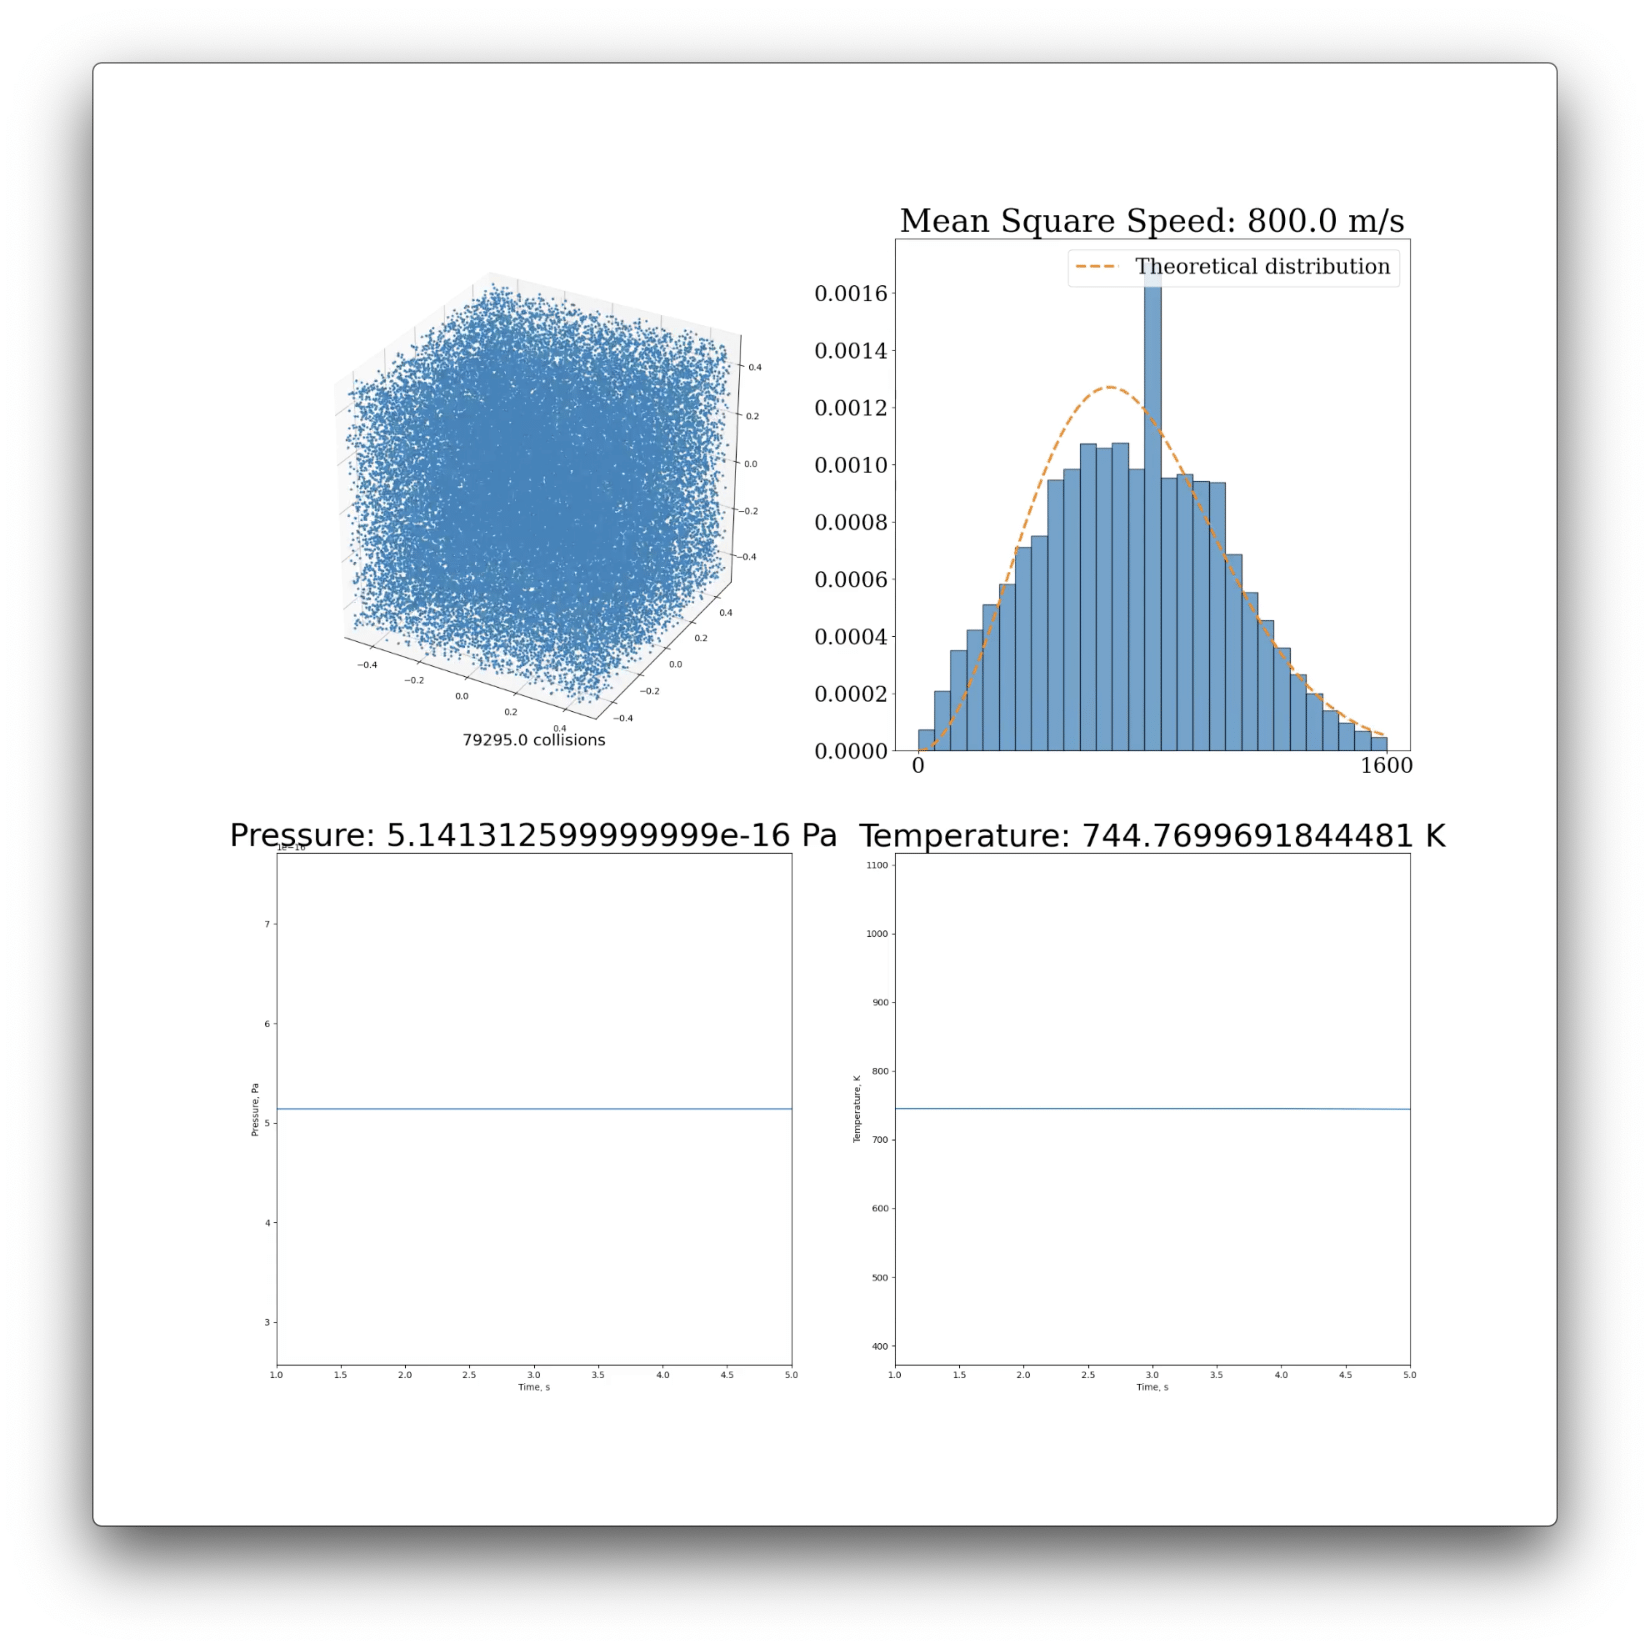
\includegraphics[width=0.57\linewidth]{Materials/eng_materials/UI}}
        \caption{There are actual states of the system at a specific time: A) Gas molecules in a vessel, B) Speed distibution 
        C) The pressure in the vessel D) The temperature in the vessel }
    \end{figure}
  
    \begin{figure}[H]
        \centering
        {\includegraphics[width=0.45\linewidth]{Materials/graphs/particles-1}}
        \caption{Cubic vessel with the final positions of the particles and their speed. 
        The faster the particle is, the closer its color is to red (blue particles are slower, than the red ones)}
    \end{figure}

    There is some problem which prevents the detection of the collision of two particles: the velocities of molecules are too high 
    and the intermediate collisions of particles can not be defined during the simulation step $dt$.
    Therefore, it should be said that the particles are considered to collide if after the passage of time they were at a small fixed distance $d(\sim 10^{-7})$ m.
    So, the fact of collision, is set by considering particles final positions.

    The following design was chosen for application architecture project:

    \begin{figure}[H]
        \centering
        {\includegraphics[width=0.65\linewidth]{Materials/eng_materials/architectura}}
        \caption{The scheme above is a software architecture of the code. Python is used to begin the simulation and to collect the report.
        There are several arguments that are sent to the program input: number of particles(\textbf{particles}), duration of the simulation(\textbf{simulation}),
        initial speed of molecule(\textbf{speed}), location of the engine in C++(\textbf{engine}). The engine is written in C++.}
    \end{figure}

    So these are the actions to run the simulation:
    \begin{enumerate}
        \item Build C++ project using next command: \\ \em{g++ -O3 -o simulation -Wno-write-strings -std=c++17 main.cpp}
        \item Use python3 to run render.py file by next command: 
        \em{python3 render.py --engine ../cmake-build-debug/gas\_simulation --particles 1000 --duration 10 --speed 800}
    \end{enumerate}

    \subsection{Execution time}

  The simulation program was run on the following machines: 
\begin{itemize}
    \item Apple MacBook Pro 13inch 2019.
    \item Yandex compute cloud machine with Intel Cascade Lake Platfrom with 32 VCPU and 128 RAM.
\end{itemize}

Detailed characteristics of yandex cloud machine and the comparison of performance are presented below.

    \begin{figure}[H]
        \centering
        {\includegraphics[width=0.6\linewidth]{Materials/eng_materials/yandex_cloud}}
        \caption{Configuring a virtual machine on yandex compute cloud which was used for run simulation. 
        } 
    \end{figure}

    \begin{figure}[H]
        \centering
        {\includegraphics[width=0.7\linewidth]{Materials/eng_materials/ex_time}}
        \caption{Scheme demostrates the dependence of the execution time and number of particles. There were two machines that had been used to run simulation: 
        Macbook Pro, Yandex computer cloud with 32 vCPU and 128 RAM.}
    \end{figure}

    \section{Results}
    Let's continue with processing gathered results, checking the ideal gas law, constructing and testing the velocity distribution hypothesis,
    looking at the pressure fluctuation, as well as the energy distribution of particles, adding the acceleration of free fall.

    \subsection{Ideal gas law}
    \indent Now the ideal gas law is going to be derived. 
    The pressure $P$ on the wall will be found using simulation and compared with the result of Ideal gas law \cite{wiki:idealgas}:
    \begin{equation}
        PV = \nu R T
    \end{equation}

    \begin{table}[H]
        \centering
        \label{Table 1}
        \begin{tabular}{|l|l|l|l|l|}
            \hline
            \multicolumn{1}{|c|}{ $T$, $K$ } & \multicolumn{1}{c|}{$V$, $\frac{m}{s}$ } & \multicolumn{1}{c|}{$N$ } & \multicolumn{1}{c|}{$P$, $10^{-17}$ } & \multicolumn{1}{c|}{$P$, $10^{-17}$ }  \\
            \hline
            $104.69$                        & $1$                                       & $7\cdot 10^3$             & $1.01$                                & $1.01$                                 \\
            \hline
            $186.95$                         & $1$                                       & $10^4$                    & $2.58$                                & $2.58$                                 \\
            \hline
            $291.25$                         & $1$                                       & $10^4$                    & $4.02$                                & $4.02$                                 \\
            \hline
            $418.00$                         & $1$                                       & $10^4$                    & $5.79$                                & $5.77$                                 \\
            \hline
            $570.43$                         & $1$                                       & $10^4$                    & $7.88$                                & $7.88$                                 \\
            \hline
            $104.62$                         & $1$                                       & $10^4$                    & $1.44$                                & $1.44$                                 \\
            \hline
            $104.63$                         & $0.729$                                   & $10^4$                    & $1.98$                                & $1.98$                                 \\
            \hline
            $104.63$                         & $0.512$                                   & $10^4$                    & $2.82$                                & $2.82$                                 \\
            \hline
            $104.63$                         & $0.343$                                   & $10^4$                    & $4.2$                                 & $4.21$                                 \\
            \hline
            $104.63$                         & $0.216$                                   & $10^4$                    & $6.7$                                 & $6.69$                                 \\
            \hline
            $104.63$                         & $0.125$                                   & $10^4$                    & $11.5$                                & $11.56$                                \\
            \hline
            $104.95$                         & $1$                                       & $2 \cdot 10^4$            & $2.9$                                 & $2.90$                                 \\
            \hline
        \end{tabular}
        \caption{Сomparing the wall pressure that is got by using the model with theory results.
        The pressure of simulated ideal gas corresponds well with theoretical $PV = N K_B T / V$ prediction.}
    \end{table}

    \subsection{Maxwell distribution}

    \textbf{Theory: }

    \indent The Maxwell–Boltzmann distribution is a result of kinetic theory of gases,
    which provides a simplified explanation of many fundamental gaseous properties, including pressure and diffusion \cite{aldor2013power}.
    It applies fundamentally to particle velocities in three dimensions, but turns out to depend only on the speed (the magnitude of the velocity) of the particles.

    \indent A particle speed probability distribution indicates which speeds are more likely: a particle will have a speed selected randomly from the distribution,
    and is more likely to be within one range of speeds than another. The kinetic theory of gases applies to the classical ideal gas, which is an idealization of real gases.
    In real gases, there are various effects (e.g., van der Waals interactions, vortical flow, relativistic speed limits, and quantum exchange interactions)
    that can make their speed distribution differ from the Maxwell–Boltzmann form. However, rarefied gases at ordinary temperatures behave nearly like an ideal gas
    and the Maxwell speed distribution is an excellent approximation for such gases.

    In the given case the following distribution should be observed:

      \begin{equation}
        p(\upsilon) = 4\pi\upsilon^2 \Big( \dfrac{m}{2\pi kT} \Big)^{3/2}\cdot e^{-\dfrac{m \upsilon^2}{2kT}}
    \end{equation}

    \textbf{Results: }

    \indent In this way, one of the most important parts of this work was to verify the establishment of the Maxwell distribution.
    That is why the initial parameters of the simulation were selected to be $100,000$ molecules of a monatomic gas with the mass of the molecule $4.82 \cdot 10^{-26}$ kg,
    in the vessel having the shape of a cube with a side $1$,
    Molecules were given initially the same modulus of speed, equal to $800$ m/s.
    After a few seconds of simulation the desired distribution has been established.

    Here are the graphs obtained on the basis of calculations:

    \begin{figure}[H]
        \centering
        {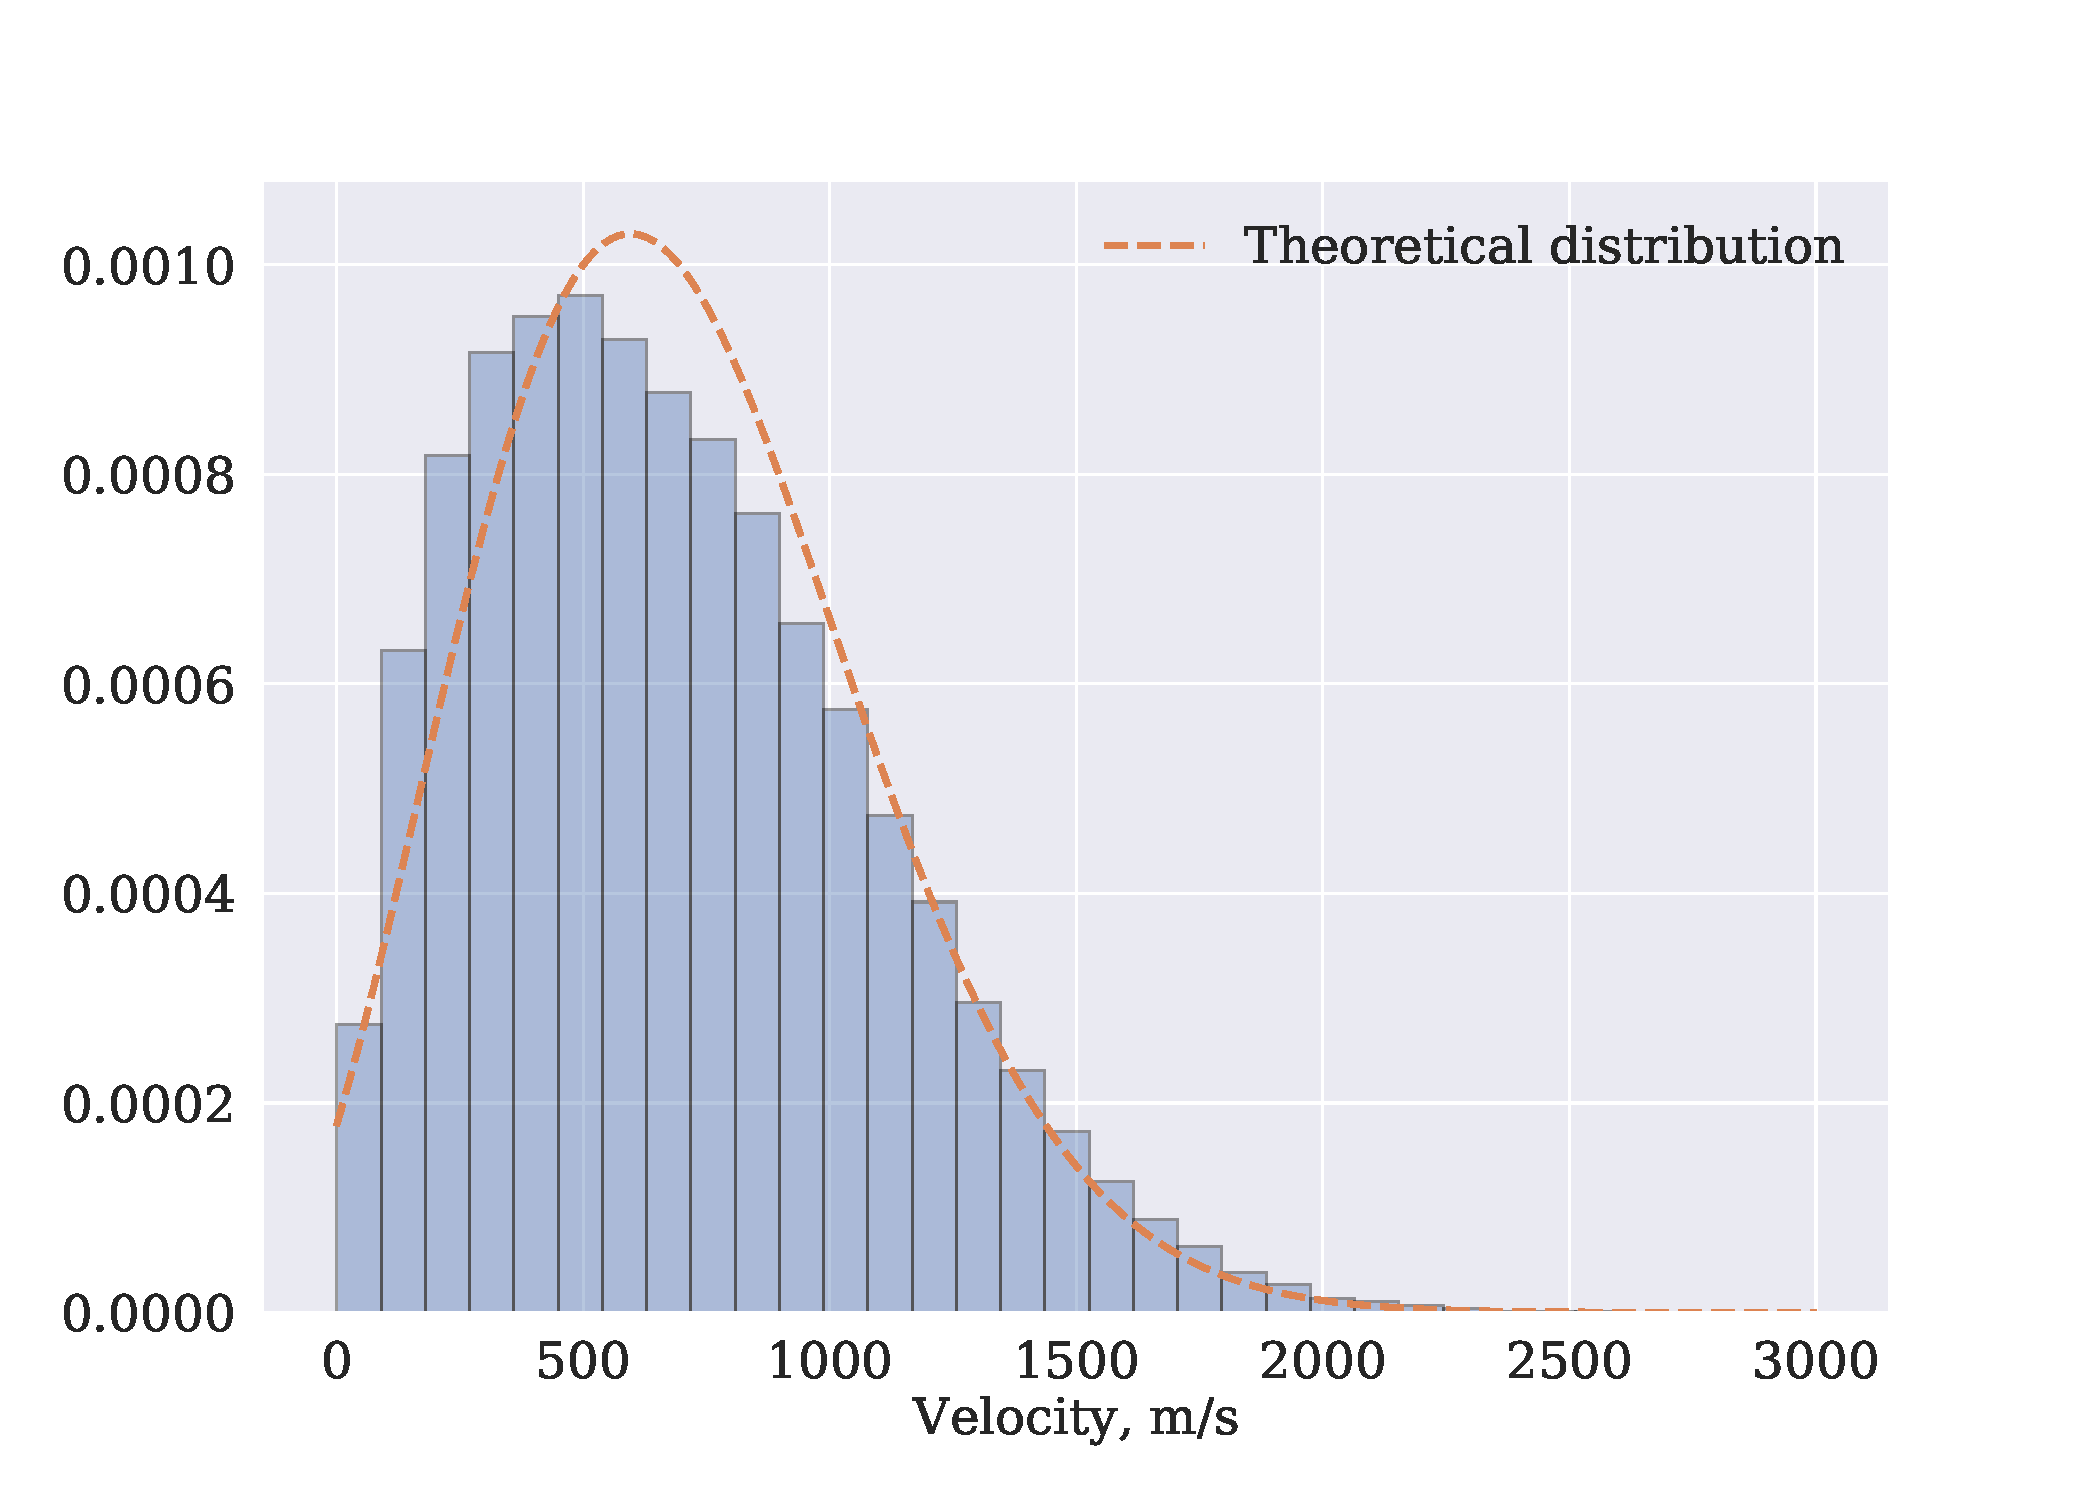
\includegraphics[width=0.7\linewidth]{Materials/eng_materials/hist_v}}
        \caption{Distribution of the fraction of molecules $\Big(\dfrac{dn}{n} (\upsilon) \Big)$ on velocity. \textit{Dotted line} the theoretical distribution is indicated. }
    \end{figure}

    \subsubsection{Hypothesis testing: Maxwell distibution}

    Let's check whether the sample obtained from the absolute velocities of molecules is really a sample from the Maxwell distribution.
    The fact that distribution coincides with the theoretical one is now going to be mathematically proven. In order of this, Kolmogorov criterion \cite{kolmogorov1933sulla} is going to be used.
    The Kolmogorov–Smirnov statistic quantifies a distance between the empirical distribution function of the sample and the cumulative distribution function of the reference distribution.
    The null distribution of this statistic is calculated under the null hypothesis so that is why the sample is taken from the theoretical distribution.

    The critical region of the Kolmogorov test is calculated using the formula:
    \begin{equation}
        \sqrt{n} \cdot \sup\limits_{x \in R} \| \hat{F_n}(x)- F_0(x) \| > K_{1-\alpha}.
    \end{equation}

    The hypothesis that the resulting distribution is a Maxwell distribution is going to be tested with parameters gathered by the maximum likelihood method.
    $p-value$ of the resulting criterion is almost zero, so the model still has an error, and it can not be said that the resulting distribution exactly matches the Maxwell distribution.
    Well, statistically significant result was got, but what can be said about practical significance?


    \indent The fact that Kolmogorov's criterion rejected hypothesis is true, the difference is appeared in distributions on the graphs, and taking into account the size of a sample,
    the power of the criterion is almost equal to one.

    Formal goodness-of-fit tests are available and quite powerful, but only indicate whether there is a lack of fit and do not explain why it is so.
    It seems that the distribution is still very close to the Maxwellian distribution, it means that the difference is almost insignificant.
    To make sure of this, let's build Q-Q plot that is often used in statistics \cite{aldor2013power}.
    The more it looks like a straight line, the closer the sample and theoretical distributions are.

    \begin{figure}[H]
        \centering
        {\includegraphics[width=0.7\linewidth]{Materials/eng_materials/qqplot}}
        \caption{Q-Q plot. Graphical method of comparing two probability distributions by plotting their quantiles against each other %check 
        }
    \end{figure}

    \textbf{Conclusion:}

    According to the schedule, it is similar to a straight line.
    There is a slight offset near zero, in fact it means that the distribution has a Maxwellian appearance, slightly inflated at zero.
    So, using Q-Q plot, it is obvious that the distribution is very close to Maxwell.

    \subsection{Hypothesis testing:Pressure fluctuations}

    From the course of General physics it is known, that fluctuations in the parameters of a thermodynamic system have the form of a normal distribution. \cite{sivuhin}

    Fluctuations, such as volume or temperature, are often considered. Fluctuations in pressure are rarely considered, since in practice.
    They are almost impossible to measure. When the concentration of molecules increases, the dispersion of pressure distribution over time, according to
    to the Central limit theorem \cite{rosenblatt1956central}, has a root rate of convergence to the mean.
    The actual obtained pressure fluctuations is negligible, but the unique chance is given to consider these fluctuations, since the pressure is simply known, and there is no need to measure it with any device.

    \begin{figure}[H]
        \centering
        {\includegraphics[width=0.7\linewidth]{Materials/eng_materials/hist_p}}
        \caption{Histogram of the pressure distribution on the vessel walls over time which was set after a few seconds of simulation.}
    \end{figure}

    From the graph it is seen that the distribution is exactly normal. The maximum likelihood estimation gives
    average value $\mu = 3.0848 \cdot 10^{-16}$ PA, variance $\sigma = 9.1215 \cdot 10^{-20}$ PA. Let's test the hypothesis that
    the resulting sample is actually from this distribution. Let's use again the Kolmogorov criterion that was considered earlier with the level of
    the value is $0.05$. The $p-value = 0.5074 > \alpha = 0.05$ is got, so, the hypothesis that the pressure distribution is
    the normal distribution with the parameters $\mu$ and $\sigma^2$ was not rejected.

    \subsection{Energy distribution in the field of gravity}

    In addition, the distribution of energy in the field of potential forces is going to be considered.
    For example, considering a system in which the Maxwellian velocity distribution is established, consisting of $100,000$ particles in a cube $1 \times 1 \times 1$ m at a temperature of 744.7 K, in the field of gravity.

    \indent The figure shows a histogram of energy distributions after 10 seconds of simulation time. As it can be seen,
    the dependence of the fraction of particles and energy is exponential, and it can be assumed that it is a Boltzmann distribution that
    is a subspecies of exponential. Let's test the hypothesis that received energies have an exponential distribution.
    Let’s calculate the parameters of this distribution by the maximum likelihood method. Indeed, using the Anderson-darling test, it is seen that with a probability of $0.985$, the energy is distributed
    exponentially.

    \begin{figure}[H]
        \centering
        {\includegraphics[width=0.6\linewidth]{Materials/eng_materials/hist_E}}
        \caption{Distribution of the fraction of molecules $\Big(\dfrac{dn}{n} (\upsilon) \Big)$ 
        according to the energy received after a long period of time.}
    \end{figure}

    \subsection{Heat machine cycle}
    Also let's try to simulate the heat engine thermodynamic cycle\cite{wiki:heatmachine}.
    The cycle will consist of adiabatic compression (isentropic process), isochoric cooling, isothermal expansion, and isochoric heating.

    Adiabatic equation for an ideal gas:
    \begin{equation}
        PV^\gamma = const
    \end{equation}

    Then knowing the starting point $P_0, V_0$ it is not difficult to plot $P(V)$ graph:
    
    $P = \dfrac{P_0 V_0^\gamma}{V ^\gamma}, \text{ where } \gamma = \dfrac{5}{3} \text{(monatomic gas)}.    $
    
    The isotherm equation is obtained from the equality:
    \begin{equation}
        PV = const \Rightarrow P = \dfrac{P_1 V_1}{V}.
    \end{equation}

    \begin{figure}[H]
        \centering
        {\includegraphics[width=1\linewidth]{Materials/eng_materials/cycle_graphs}}
        \caption{Experimental and theoretical graphs of the heat machine cycle in $PV$ coordinates. 
        The heat machine cycle consists of the following processes
        1) Adiabatic compression 2) Isochoric cooling 3) Isothermal expansion 4) Isochoric heating .}
    \end{figure}

    \textbf{Conclusion:}
    In this way, an almost perfect correspondence between the experimental and theoretical results was obtained, despite the fact that
    each process had been performed just for $10$ seconds.
    The model describes a monatomic ideal gas with high accuracy. It allows to conduct processes over it and simulate a heat engine.

    \section{Conclusion}
    
    \indent In summary, the validity of the model seems to be convincing. 
    The basic law of thermodynamic was tested and the core principles of statistical mechanics were demonstrated.
    Firstly, the ideal gas law ($P V = N k_B T$) was proven by measuring the pressure as function of $V$, $N$, $k_B T$ and it was found that the model corresponds to the monatomic gas.
    Secondly, the hypothesis that molecules velocities are distributed by Maxwell was tested.
    Thirdly, the normality of pressure fluctuations was confirmed.
    And finally, the cycle of the heat engine was simulated and the exact result was gathered.
    \bibliographystyle{plain}
    \bibliography{bibliography}

\end{document}
